
\section{Das Android Betriebssystem}
	Das Unternehmen Android wurde 2003 von Andy Rubin gegründet und wurde 2005 von Google aufgekauft. Seitdem kümmert sich Google und das Android Open Source Project (AOSP) um die Weiterentwicklung des Systems. Zuletzt wurden die neuen Versionen jeweils von Google intern entwickelt und zum Release der Version der AOSP Community als Open-Source bereitgestellt. Das Betriebssystem wird in den meisten Fällen von den Smartphone Herstellern, oder Entwicklerteams, noch weiter angepasst, bevor es für die einzelnen Geräte bereitgestellt wird.\\
	Aktuell ist Android, mit 55.6\% Marktanteil \cite{MobileOsStat}, das vorherrschende Betriebssystem für mobile Endger"ate in den USA.
	\\\\
	Basis für das Betriebssystem ist ein modifizierter Linux-Kernel und eine Java Virtual Machine (JVM). Bis einschliesslich Version 4.4 wurde hierfür die Dalivk Runtime und für alle neueren Versionen die Android Runtime (ART) verwendet. Jede App l"auft in einer eigenen Instanz der entsprechenden Runtime und damit in einer Sandbox.\newline
	Oberhalb der JVM sind die meisten Komponenten in Java implementiert.\\
	
	\begin{figure}[h]
		\centering
		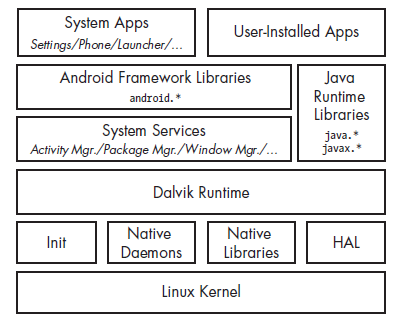
\includegraphics[width=0.7\linewidth]{android_pages/graphics/architektur_android_.png}
		\caption{Die Android Architektur \protect\cite{Elenkov2014} }
		\label{fig:architektur_android}
	\end{figure}